\documentclass[13pt]{beamer}
%
% Choose how your presentation looks.
%
% For more themes, color themes and font themes, see:
% http://deic.uab.es/~iblanes/beamer_gallery/index_by_theme.html
%
\mode<presentation>
{
\usetheme{CambridgeUS}     % or try Darmstadt, Madrid, Warsaw, ...
\usecolortheme{beaver} % or try albatross, beaver, crane, ...
\usefonttheme{default}  % or try serif, structurebold, ...
\setbeamertemplate{navigation symbols}{}
\setbeamertemplate{caption}[numbered]
} 

\usepackage[english]{babel}
\usepackage[utf8x]{inputenc}
\usepackage{xcolor}
\usepackage{multicol}
\usepackage{tikz}
\usepackage{tikz-uml}
\tikzumlset{font=\footnotesize\ttfamily}
\usepackage{hyperref}

\usepackage{listings}
\definecolor{codegreen}{rgb}{0,0.6,0}
\definecolor{codegray}{rgb}{0.5,0.5,0.5}
\definecolor{codepurple}{rgb}{0.58,0,0.82}
\definecolor{backcolour}{rgb}{0.95,0.95,0.92}

\lstdefinestyle{myCustomCppStyle}{
language=C++,
numbers=left,
stepnumber=1,
numbersep=9pt,
tabsize=2,
showspaces=false,
showstringspaces=false
}

\lstset{basicstyle=\tiny,style=myCustomCppStyle}

\lstdefinestyle{mystyle}{
backgroundcolor=\color{backcolour},   
commentstyle=\color{codegreen},
keywordstyle=\color{magenta},
numberstyle=\tiny\color{codegray},
stringstyle=\color{codepurple},
basicstyle=\ttfamily\footnotesize,
breakatwhitespace=false,         
breaklines=true,                 
captionpos=b,                    
keepspaces=true,                 
numbers=left,                    
numbersep=5pt,                  
showspaces=false,                
showstringspaces=false,
showtabs=false,                  
tabsize=1
}

\lstset{style=mystyle}

\usepackage{graphicx}
\graphicspath{ {./images/} }

\usepackage{tikz}
\usetikzlibrary{decorations.text}
\usetikzlibrary{shapes.geometric, arrows, positioning, calc, matrix}

\tikzset{
basic box/.style={
shape=rectangle, rounded corners, align=center,
draw=#1, fill=#1!25},
header node/.style={
Minimum Width=header nodes,
font=\strut\Large\ttfamily,
text depth=+0pt,
fill=white, draw},
header/.style={%
inner ysep=+1.5em,
append after command={
\pgfextra{\let\TikZlastnode\tikzlastnode}
node [header node] (header-\TikZlastnode) at (\TikZlastnode.north) {#1}
node [span=(\TikZlastnode)(header-\TikZlastnode)] at (fit bounding box) (h-\TikZlastnode) {}
}
},
hv/.style={to path={-|(\tikztotarget)\tikztonodes}},
vh/.style={to path={|-(\tikztotarget)\tikztonodes}},
fat blue line/.style={ultra thick, blue}
}

\definecolor{mygray}{RGB}{208,208,208}
\definecolor{mymagenta}{RGB}{226,0,116}
\newcommand*{\mytextstyle}{\sffamily\Large\bfseries\color{black!85}}
\newcommand{\arcarrow}[3]{%
% inner radius, middle radius, outer radius, start angle,
% end angle, tip protusion angle, options, text
\pgfmathsetmacro{\rin}{1.7}
\pgfmathsetmacro{\rmid}{2.2}
\pgfmathsetmacro{\rout}{2.7}
\pgfmathsetmacro{\astart}{#1}
\pgfmathsetmacro{\aend}{#2}
\pgfmathsetmacro{\atip}{5}
\fill[mygray, very thick] (\astart+\atip:\rin)
             arc (\astart+\atip:\aend:\rin)
-- (\aend-\atip:\rmid)
-- (\aend:\rout)   arc (\aend:\astart+\atip:\rout)
-- (\astart:\rmid) -- cycle;
\path[
decoration = {
text along path,
text = {|\mytextstyle|#3},
text align = {align = center},
raise = -1.0ex
},
decorate
](\astart+\atip:\rmid) arc (\astart+\atip:\aend+\atip:\rmid);
}
\title[Design Pattern]{Structural Design Pattern}
\author{Hung Tran}
\institute{Fpt software}
\date{\today}


\begin{document}

\begin{frame}
	\titlepage
\end{frame}

% Uncomment these lines for an automatically generated outline.
\begin{frame}{Outline}
	\tableofcontents
\end{frame}

\section{Structural Pattern Overview}

\begin{frame}{Structural Pattern Overview}
	\begin{center}
		\textcolor{blue}{\textbf{How classes and objects are composed to form larger structure.}}
	\end{center}
	\begin{itemize}
		\item \textbf{Adapter}: Convert the interface of a class into another interface.
		\item \textbf{Bridge}: Decouple an abstraction from its implementation.
		\item \textbf{Composite}: Compose objects into tree structure.
		\item \textbf{Decorator}: Attach additional responsibilities to an object dynamically.
		\item \textbf{Facade}: Provide a unified interface to a set of interfaces.
		\item \textbf{Flyweight}: Use sharing to support large numbers of fine-grained objects efficiently.
		\item \textbf{Proxy}: Provide a surrogate or placeholder for another object to control access to it.
	\end{itemize}
\end{frame}

\section{Bridge design pattern}

\begin{frame}{Problem Statement}
	\begin{columns}[T]
		\begin{column}{.5\textwidth}
			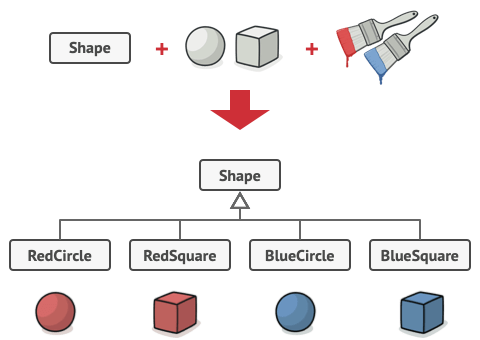
\includegraphics[scale=0.4]{./images/problem.png}
		\end{column}
	
		\begin{column}{.4\textwidth}
			\begin{itemize}
				\item You have a geometric Shape class with a pair of subclasses: Circle and Square.
				\item You want to extend this class hierarchy to incorporate colors.
				\item Adding new shape types and colors to the hierarchy will grow it exponentially.
				\item The total classes by combination?
			\end{itemize}
		\end{column}
	\end{columns}
\end{frame}

\begin{frame}{Problem Statement}
	\begin{columns}[T]
		\begin{column}{.5\textwidth}
			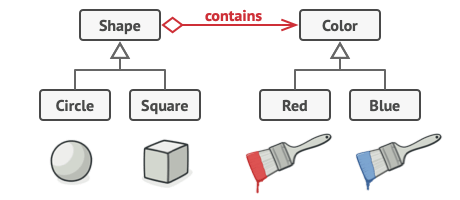
\includegraphics[scale=0.45]{./images/solution.png}
		\end{column}
	
		\begin{column}{.4\textwidth}
			\begin{itemize}
				\item The Bridge pattern attempts to solve this problem by switching from inheritance to the object composition.
				\item Adding new colors won’t require changing the shape hierarchy, and vice versa.
			\end{itemize}
		\end{column}
	\end{columns}
\end{frame}

\begin{frame}{The Intent of Bridge Design Pattern}
	\begin{center}
	\textcolor{red}{\textbf{Decouple an abstraction from its implementation so that the two can vary independently.}}
	\end{center}
\end{frame}

\begin{frame}{Structure of Bridge Pattern: Object adapter}
	\begin{center}
		\begin{tikzpicture}
			\umlemptyclass[x=0,y=0]{Client}
			\umlclass[x=3,y=0]{Abstraction}{}{operation()}
			\umlclass[x=2,y=-4]{RefinedAbstruction}{}{}
			\umlclass[x=8,y=0]{Implementor}{}{operationImp()}
			\umlclass[x=6,y=-4]{ConcreteA}{}{operationImp()}
			\umlclass[x=10,y=-4]{ConcreteB}{}{operationImp()}
			\umluniaggreg{Abstraction}{Implementor}
			\umluniassoc[pos=0.95, align=right, name=uniassoc]{Client}{Abstraction}
			\umlinherit[geometry=|-|]{RefinedAbstruction}{Abstraction}
			\umlinherit[geometry=|-|]{ConcreteA}{Implementor}
			\umlinherit[geometry=|-|]{ConcreteB}{Implementor}
		\end{tikzpicture}	
	\end{center}
\end{frame}

\begin{frame}{Pointer to Implementation (PIMPL)}
	\textcolor{blue}{}
	\begin{itemize}
		\setlength\itemsep{1em}
		\item PIMPLE is the manifestation of the bridge design pattern albeit a slightly different one.
		\item PIMPL idiom is all about hiding the implementation details of a particular class by sticking it into separate implementation pointed by pointer just as the name suggests.
	\end{itemize}
\end{frame}

\begin{frame}{PIMPL implementation}
\begin{columns}[T]
\begin{column}{.45\textwidth}
\lstset{basicstyle=\tiny,style=myCustomCppStyle}
person.h
\lstinputlisting{./examples/pimpl/person.h}
\end{column}

\begin{column}{.45\textwidth}
\lstset{basicstyle=\tiny,style=myCustomCppStyle}
person.cpp
\lstinputlisting{./examples/pimpl/person.cpp}
\end{column}
\end{columns}
\end{frame}

\begin{frame}{Why would you want to do this PIMPL?}
	\textcolor{blue}{}
	\begin{itemize}
		\setlength\itemsep{1em}
		\item Security purpose: a data member which contains critical information.
		\item Compilation time
	\end{itemize}
\end{frame}

\begin{frame}{Disadvantages of PIMPL?}
	\textcolor{blue}{}
	\begin{itemize}
		\setlength\itemsep{1em}
		\item Run-time overhead as we have to dereference the pointer every time for access.
		\item Construction \& destruction overhead of unique\_ptrbecause it creates a memory in a heap
		\item We also have to bear some indirection if we want to access the data member of Person in PersonImpl like passing this pointer or so
	\end{itemize}
\end{frame}

\begin{frame}{Applicability}
	\textcolor{blue}{}
	\begin{itemize}
		\item Use the Bridge pattern when you want to divide and organize a monolithic class that has several variants of some functionality (for example, if the class can work with various database servers).
		\item The bigger a class becomes, the harder it is to figure out how it works, and the longer it takes to make a change. The changes made to one of the variations of functionality may require making changes across the whole class, which often results in making errors or not addressing some critical side effects.
		\item The Bridge pattern lets you split the monolithic class into several class hierarchies. After this, you can change the classes in each hierarchy independently of the classes in the others. This approach simplifies code maintenance and minimizes the risk of breaking existing code.
	\end{itemize}
\end{frame}

\begin{frame}{Applicability}
	\textcolor{blue}{}
	\begin{itemize}
		\item Use the pattern when you need to extend a class in several orthogonal (independent) dimensions.
		\item The Bridge suggests that you extract a separate class hierarchy for each of the dimensions. The original class delegates the related work to the objects belonging to those hierarchies instead of doing everything on its own.
		\item Use the Bridge if you need to be able to switch implementations at runtime.
		\item Although it’s optional, the Bridge pattern lets you replace the implementation object inside the abstraction. It’s as easy as assigning a new value to a field.
		%By the way, this last item is the main reason why so many people confuse the Bridge with the Strategy pattern. Remember that a pattern is more than just a certain way to structure your classes. It may also communicate intent and a problem being addressed.
	\end{itemize}
\end{frame}

\begin{frame}{How to Implement}
	\begin{itemize}
		\item Identify the orthogonal dimensions in your classes. These independent concepts could be: abstraction/platform, domain/infrastructure, front-end/back-end, or interface/implementation.
		\item See what operations the client needs and define them in the base abstraction class.
		\item Determine the operations available on all platforms. Declare the ones that the abstraction needs in the general implementation interface.
		\item For all platforms in your domain create concrete implementation classes, but make sure they all follow the implementation interface.
	\end{itemize}
\end{frame}

\begin{frame}{How to Implement}
	\begin{itemize}
		\item Inside the abstraction class, add a reference field for the implementation type. The abstraction delegates most of the work to the implementation object that’s referenced in that field.
		\item If you have several variants of high-level logic, create refined abstractions for each variant by extending the base abstraction class.
		\item The client code should pass an implementation object to the abstraction’s constructor to associate one with the other. After that, the client can forget about the implementation and work only with the abstraction object.
	\end{itemize}
\end{frame}

\begin{frame}{Pros and Cons}
	\begin{columns}[T]
		\begin{column}{.5\textwidth}
			\begin{itemize}
				\item You can create platform-independent classes and apps.
				\item The client code works with high-level abstractions. It isn’t exposed to the platform details.
				\item Open/Closed Principle. You can introduce new abstractions and implementations independently from each other.
				\item Single Responsibility Principle. You can focus on high-level logic in the abstraction and on platform details in the implementation.
			\end{itemize}
		\end{column}
	
		\begin{column}{.5\textwidth}
			\begin{itemize}
				\item  You might make the code more complicated by applying the pattern to a highly cohesive class.
			\end{itemize}
		\end{column}
	\end{columns}
\end{frame}

\begin{frame}{Relations with Other Patterns}
	\begin{itemize}
		\item Bridge is usually designed up-front, letting you develop parts of an application independently of each other. On the other hand, Adapter is commonly used with an existing app to make some otherwise-incompatible classes work together nicely.
		\item Bridge, State, Strategy (and to some degree Adapter) have very similar structures. Indeed, all of these patterns are based on composition, which is delegating work to other objects. However, they all solve different problems. A pattern isn’t just a recipe for structuring your code in a specific way. It can also communicate to other developers the problem the pattern solves.
		\item You can use Abstract Factory along with Bridge. This pairing is useful when some abstractions defined by Bridge can only work with specific implementations. In this case, Abstract Factory can encapsulate these relations and hide the complexity from the client code.
		\item You can combine Builder with Bridge: the director class plays the role of the abstraction, while different builders act as implementations.
	\end{itemize}
\end{frame}

\begin{frame}
\begin{center}
{\fontsize{40}{50}\selectfont Thank You!}
\end{center}
\end{frame}


\end{document}
